%==============================================================================
% Voorbeeld hogent-article: onderzoeksvoorstel bachproef
%==============================================================================

\documentclass{hogent-article}

\usepackage{lipsum} % Voor vultekst

% Invoegen bibliografiebestand
\addbibresource{references.bib}

% Informatie over de opleiding, het vak en soort opdracht
\studyprogramme{Professionele bachelor toegepaste informatica}
\course{Bachelorproef}
\assignmenttype{Paper: Onderzoeksvoorstel}
\academicyear{2023-2024} % TODO: pas het academiejaar aan

% TODO (fase 1): Werktitel
\title{Welke rendermodus is het meest geschikt voor het ontwikkelen van webapplicaties met betrekking tot laadtijd, netwerkprestaties, zoekmachineoptimalisatie en schaalbaarheid in .NET 8?}

% TODO (fase 1): Studentnaam en emailadres invullen
\author{Jeff Wellekens}
\email{jeff.wellekens@student.hogent.be}

% TODO (fase 1): Medestudent
% Schrijf je het voorstel in samenwerking met een medestudent? Geef dan de naam
% en emailadres hier. Als je het voorstel alleen schrijft, verwijder dan deze
% regels of zet ze in commentaar.
% \author{}
% \email{}

% TODO (fase 1): Geef hier de link naar jullie Github-repository
\projectrepo{https://github.com/jeffwellekens/bp-voorstel}

% Binnen welke specialisatierichting uit 3TI situeert dit onderzoek zich?
% Kies uit deze lijst:
%
% - Mobile \& Enterprise development
% - AI \& Data Engineering
% - Functional \& Business Analysis
% - System \& Network Administrator
% - Mainframe Expert
% - Als het onderzoek niet past binnen een van deze domeinen specifieer je deze
%   zelf
%
\specialisation{Mobile \& Enterprise development}
% Geef hier enkele sleutelwoorden die je onderwerp beschrijven
\keywords{.NET 8, Blazor, Client-Side Rendering, Server-side rendering}

\begin{document}

\begin{abstract}
  % performantie is te algemeen dit moet concreter worden beschreven (laadtijd, ...)
  Deze paper onderzoekt welke rendermodus het meest geschikt is in .NET 8 op basis
  van laadtijd, netwerkprestaties, zoekmachineoptimalisatie en schaalbaarheid voor het creëren van webapplicaties. 
  Het doel van dit onderzoek is om softwareontwikkelaars te voorzien van een duidelijk inzicht in de voordelen en nadelen van
  elke rendermodus, zodat zij doordachte keuzes kunnen maken bij het selecteren van een rendermodus. Allereerst zal er een grondige literatuurstudie 
  worden uitgevoerd om inzicht te verkrijgen in de verschillen tussen alle rendermodi. 
  Vervolgens zal een experiment worden uitgevoerd waarin elke rendermodi zal getest worden met een zelfgemaakte applicatie, gericht op laadtijd, netwerkprestaties, zoekmachineoptimalisatie en schaalbaarheid.
  De resulterende gegevens zullen zorgvuldig worden geïnterpreteerd om te bepalen welke rendermodus de beste keuze is op basis van de vooraf gedefinieerde criteria. 
  Er wordt verwacht uit de hypothese dat de interactive server rendermodus de beste resultaten zal vertonen op basis van van laadtijd, netwerkprestaties, zoekmachineoptimalisatie en schaalbaarheid. Desondanks
  dat de interactive server rendermodus de beste resultaten zal opleveren volgen de hypothese zal er ook blijken dat er gebruik kan gemaakt worden van de interactive webassembly rendermodus voor aan
  de schaalbaarheid criteria te voldoen op component niveau. 
\end{abstract}

\tableofcontents

\bigskip

% TODO: Neem je dit jaar ook de bachelorproef op? Haal dan de tekst hieronder
% uit commentaar en pas het aan.

%\paragraph{Opmerking}

% Ik neem dit jaar ook de bachelorproef op. De inhoud van dit onderzoeksvoorstel dient ook als het onderwerpvoor mijn bachelorproef. Mijn promotor is (Mr./Mevr.) X.\ Familienaam.

% Beschrijf de eventuele verschillen en/of verbeteringen in dit document t.o.v.\ jouw onderzoeksvoorstel dat je ingediend hebt voor de bachelorproef.

\section{Inleiding}%
\label{sec:inleiding}

% TODO: (fase 1) introduceer je gekozen onderwerp, formuleer de onderzoeksvraag en deelvragen. Wat is de doelstelling (is die S.M.A.R.T.?), wat zal het resultaat zijn van het onderzoek (een Proof-of-Concept, een prototype, een advies, ...)? Waarom is het nuttig om dit onderwerp te onderzoeken?
Het algemeen onderwerp van deze paper is het vergelijken van alle rendermodi in het blazor web app template. Wanneer je als softwareontwikkelaar een 
applicatie wilt maken in het blazor framework met de nieuwe web app template in .NET 8 zal je zien dat de rendering nu kan toegekend worden per component. Deze rendering per component 
betreft de manier waarop blazor de HTML weergave zal renderen in de browser. Daarom wordt er in deze paper onderzocht welke
rendermodus de beste keuze is gebaseerd op laadtijd, netwerkprestaties, zoekmachineoptimalisatie en schaalbaarheid. De manier hoe dit zal verlopen is door middel van een experiment waarbij eenzelfde applicatie 
zal gemaakt worden met alle rendermodi. Tenslotte wanneer de metingen gebeurd en onderzocht zijn zal er advies worden gegeven over welke rendermodus het meest passend is afhankelijk van de relevante criteria.

\section{Literatuurstudie}%
\label{sec:literatuurstudie}

% TODO: (fase 4) schrijf de literatuurstudie uit en gebruik waar gepast referenties naar de vakliteratuur.
In deze literatuurstudie zullen we beginnen met het definiëren van fundamentele concepten die nodig zijn voor het begrijpen van de vakliteratuur. Vervolgens zullen we de verschillen
tussen alle rendermodi toelichten. Allereerst gaan we het hebben over client en server render concepten. De term renderen betekent het maken van de 
HTML opmaak die wordt weergegeven in de browser \autocite{Guardrex2023}.  Wat is client-side rendering (CSR)? Dit betekent dat de uiteindelijke HTML opmaak is 
gegenereerd door de blazor webassembly runtime op de client. Geen enkele HTML is hierbij verzonden van de server naar de client. Er wordt hier van uitgegaan dat er 
gebruiker interactiviteit is met de pagina. \autocite{Guardrex2023} Server-side rendering (SSR) wil zeggen dat de uiteindelijke HTML opmaak is gegenereerd door de ASP.NET Core runtime
op de server. Deze HTML wordt van de server naar de client verzonden via het netwerk om vervolgens in de browser te worden weergegeven. Server-side rendering kan bestaan uit twee
varianten. We hebben statische SSR wat betekent dat de server statische HTML creërt waarbij geen gebruiker interactie mogelijk is en ook niet het bijhouden van razor component state.
Als laatste hebben we ook interactieve SSR dit wil zeggen dat blazor events gebruiker interactiviteit toestaan en dat de razor component state wordt bijgehouden door het blazor framework. \autocite{Guardrex2023}
We gaan de client en server concepten afsluiten met een laatste definitie van prerendering. Het proces van prerendering houdt in dat initieel de pagina inhoud wordt gerenderd op de server zonder event handlers voor gerenderde controllers.
De server geeft zo snel mogelijk de HTML-gebruikersinterface terug als antwoord op het initiële verzoek. Dit zorgt ervoor dat de applicatie veel responsiever aanvoelt voor gebruikers.
Prerendering kan ook zoekmachineoptimalisatie verbeteren door de inhoud te renderen voor het initiële HTTP antwoord die zoekmachines gebruiken voor het berekenen van de website rang. \autocite{Guardrex2023}
Nu gaan we dieper in op de concepten rond statisch en interactief renderen. Een razor component kan statisch of interactief gerenderd worden \autocite{Guardrex2023}.
Statische rendering is een server-side scenario dit houdt in dat het component gerenderd wordt zonder de mogelijkheid voor interactie tussen de gebruiker en de .NET/C\# code.
Dit wil niet zeggen dat de gebruiker geen interactie meer kan hebben met de JavaScript of HTML DOM events. Het is gewoon niet mogelijk om gebruiker events die op de client gebeuren
te verwerken met .NET die op de server draait. \autocite{Guardrex2023} Daarentegen kan interactief renderen wel .NET events verwerken via C\# code. De .NET events worden verwerkt op de server door de ASP.NET Core
runtime of in de browser op de client door de WebAssembly gebaseerde runtime. \autocite{Guardrex2023} Als laatste van de fundamentele concepten bespreken we razor componenten zoals gedefinieerd door Microsoft.
\begin{quote}
  Blazor apps are based on Razor components, often referred to as just components. A component is an element of UI, such as a page, dialog, or data entry form. Components are .NET C\# classes built into .NET assemblies.
  \paragraph{}
  Razor refers to how components are usually written in the form of a Razor markup page for client-side UI logic and composition. Razor is a syntax for combining HTML markup with C\# code designed for developer productivity. Razor files use the .razor file extension. \autocite{Guardrex2023}
\end{quote}
Nu we alle fundamentele concepten besproken hebben gaan we kijken wat een rendermodus is en welke verschillende er allemaal bestaan. Elk component in een blazor web app neemt een rendermodus aan om het hosting model
dat het gebruikt te bepalen. Ook dient dit om te beslissen waar het zal gerenderd worden en of het wel of niet interactief is. \autocite{Guardrex2023a} Een rendermodus op een component kan toegekend worden door de
@rendermode directive te gebruiken bij de instantie van een component of bij de definitie ervan. \autocite{Guardrex2023a} Er zijn vier verschillende rendermodi die je kan toewijzen aan een component. Om te beginnen zullen we starten met de
Static Server rendermodus. Deze rendermodus zorgt voor static server-side rendering dit wil dus zeggen dat de rendering gebeurd op de server en hier ook geen gebruiker interactiviteit van toepassing is omdat deze rendermodus
static is \autocite{Guardrex2023a}. Daarnaast is er ook de Interactive Server rendermodus dit is hetzelfde als de vorige rendermodus maar met het verschil dat we hier wel gebruiker interactiviteit hebben door middel van een real-time connectie
met de browser. Deze connectie wordt gemaakt wanneer de server component gerenderd wordt. \autocite{Guardrex2023a} Dan hebben we ook nog de Interactive WebAssembly rendermodus deze zorgt voor client-side rendering wat ook inhoud dat deze
interactief is. De .NET runtime en app bundle worden gedownload en gecached wanner het webassembly component initieel gerenderd wordt. Belangrijk om te weten hierbij is dat componenten die client-side rendering gebruiken
in een apart client project moeten gebouwd worden dat de webassembly host instelt. \autocite{Guardrex2023a} Ten slotte hebben we de Interactive Auto rendermodus deze combineert zowel Interactive SSR als CSR. Wanneer een component met deze rendermodus
initieel wordt geladen gaat dit gebruik maken van interactive SSR. In de achtergrond wordt de .NET runtime en app bundle gedownload naar de client en gecached zodanig dat wanneer de component opnieuw bezocht wordt deze
CSR gebruikt. \autocite{Guardrex2023a} Prerendering staat standaard aan op elk interactief component \autocite{Guardrex2023a}. 
% Refereren naar de literatuur kan met:
% \autocite{BIBTEXKEY} -> (Auteur, jaartal)
% \textcite{BIBTEXKEY} -> Auteur (jaartal)

% \lipsum[4-9]

\section{Methodologie}%
\label{sec:methodologie}

% TODO: (fase 5) beschrijf in detail in welke fasen je onderzoek uiteenvalt, hoe lang elke fase duurt en wat het concrete resultaat van elke fase is. Welke onderzoekstechniek ga je toepassen om elk van je onderzoeksvragen te beantwoorden? Gebruik je hiervoor experimenten, vragenlijsten, simulaties? Je beschrijft ook al welke tools je denkt hiervoor te gebruiken of te ontwikkelen.
Als eerste zal er een grondige literatuurstudie uitgevoerd worden om fundamentele concepten uit te leggen zodat de technische definities duidelijk zijn, wanneer we de verschillen vergelijken tussen alle rendermodi die bestaan. Het resultaat dat zal opgeleverd worden is een
literatuurverslag met daarin de belangrijkste concepten en bevindingen rond rendermodi. Deze eerste fase zal twee weken duren. Ten tweede wordt er een applicatie gebouwd die nodig zal zijn om het experiment uit te voeren.
Het bouwen van deze applicatie zal twee weken duren. Als derde fase wordt het experiment uitgevoerd op de gebouwde applicatie. Dit experiment bestaat uit het meten van de laadtijd en zoekmachineoptimalisatie wat zal gebeuren door een Lighthouse
report te generen met de chrome developer tools. Ook zal er een analyse worden uitgevoerd door gebruik te maken van de netwerkfunctionaliteit in de Chrome Developer Tools. Na deze fase zal er een experimenteel verslag opgemaakt worden met daarin alle resultaten.
Vervolgens wanneer dit experimenteel verslag is gemaakt kunnen we beginnen met het analyseren van deze gegevens zodat we een beeld kunnen krijgen welke rendermodus het meest performant is gebaseerd op de vooraf gedefinieerde
criteria. Het resultaat dat we bekomen na het analyseren van deze gegevens is een rapport met daarin de belangrijkste bevindingen en interpretaties van de gegevens. Het analyseren van de gegevens zal een week tijd in beslag nemen.
Ten slotte zullen we onze conclusie baseren op dit rapport. En zo kunnen we een deskundig advies opleveren aan de softwareontwikkelaar die de nieuwe web app template van .NET 8 zal gebruiken.

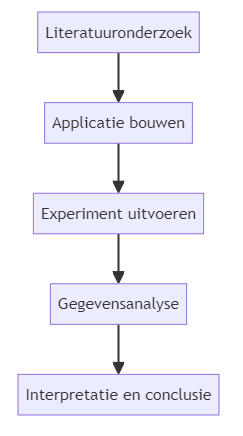
\includegraphics{img/diagram_methodologie.png}
% \lipsum[10-12]

\section{Verwachte resultaten}%
\label{sec:verwachte-resultaten}

% TODO: (fase 6) beschrijf wat je verwacht uit je onderzoek en waarom (bv. volgens je literatuuronderzoek is softwarepakket A het meest gebruikte en denk je dat het voor deze casus ook het meest geschikt zal zijn). Natuurlijk kan je niet in de toekomst kijken en mag je geen alternatieve mogelijkheden uitsluiten. In de praktijk gebeurt het ook vaak dat een onderzoek tot verrassende resultaten leidt, dat maakt het proces nog interessanter!
Volgens de hypothese wordt er verwacht dat de interactive server rendermodus zeer performant zal scoren op laadtijd, netwerkprestaties en zoekmachineoptimalisatie. Het enigste nadeel bij deze rendermodus
zal de schaalbaarheid zijn. Echter zal dit kunnen opgelost worden door gebruik te maken van verschillende rendermodi per component zodat je aan deze criteria kan voldoen op component niveau.

% \lipsum[14-18]

\section{Discussie, conclusie}%
\label{sec:discussie-conclusie}
% Herschrijven
Het nieuwe web app template van .NET 8 lijkt veel van de problemen met betrekking tot een globale render mode op te lossen. 
Door de toewijzing op componentniveau kunnen we nu beslissen welk component welke rendermodus krijgt. 
Dit geeft ons de mogelijkheid om te voldoen aan de specifieke criteria van elk afzonderlijk component. Als antwoord op de onderzoeksvraag zal het blijken dat de interactive server rendermodus de meest performante
zal zijn op basis van laadtijd, netwerkprestaties en zoekmachineoptimalisatie. Daarentegen zal de interactive webassembly rendermodus veel beter zijn wanneer er rekening moet gehouden worden met schaalbaarheid.

% \lipsum[19-21]

%------------------------------------------------------------------------------
% Referentielijst
%------------------------------------------------------------------------------
% TODO: (fase 4) de gerefereerde werken moeten in BibTeX-bestand
% bibliografie.bib voorkomen. Gebruik JabRef om je bibliografie bij te
% houden.

\printbibliography[heading=bibintoc]

\end{document}